% begin module function-machine
\begin{frame}
It is often helpful to view a function as a machine.  If $x$ is an element of $D$, then the machine takes $x$ as input and produces $f(x)$, an element of $E$, as output.

\begin{center}
\begin{pspicture}(-4, -2.5)(13,2.5)
\footnotesize
\rput[r] (-3.1, 0){$x$}
\psline[linewidth=3pt]{->}(-3,0)(-2.25,0)

\rput(0.25,0){
\fcMachine{$f$}{blue}
}
\rput (4, 0){$f(x)$}
\psline[linewidth=3pt]{->}(2.75,0)(3.5,0)
\end{pspicture}
\end{center}

%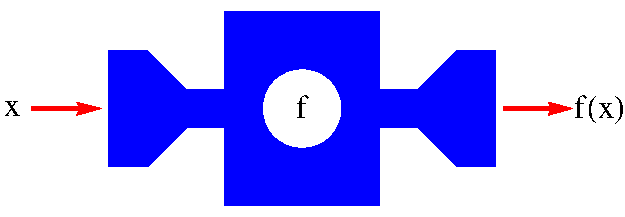
\includegraphics[height=4cm]{precalculus/pictures/01-01-machine.pdf}
\end{frame}
% end module function-machine
